\documentclass{beamer}  
\usetheme{Warsaw}
\usepackage{graphicx}
\title{Introduction to AI and ML}
\subtitle{ Matrix Project}
\author{A.AVINASH, EE17BTECH11005 \and \\K.DEVENDER, EE17BTECH11015}
\begin{document}

\begin{frame}

\titlepage
 
\end{frame}  

\begin{frame}[t]{Q.no.51 in JEE Mains(2004)}
If the lines 2x+3y+1=0 and 3x-y-4=0 lie along diameter of a circle of circumference 10\pi , 
\ $then the equation of the circle is$

\end{frame}
\begin{frame}
Given line equation is $2x+3y+1=0$ 
\newline
\newline
Line equation in matrix form 
\begin{bmatrix}
2 & 3 \\
\end{bmatrix}\textbf{X}
= -1 \hspace{10mm} \textbf{(1)}
\newline
\newline
Given line equation is $3x-y-4=0$ 
\newline
\newline
Line equation in matrix form 
\begin{bmatrix}
3 & -1 \\
\end{bmatrix}\textbf{X}
= 4 \hspace{10mm} \textbf{(2)}
\end{frame}
\begin{frame}
As given two lines lie along the diameters of the circle, so thier intersection point is the centre of the circle
\newline
\newline
Solving equation \textbf{(1)} and\textbf{(2)}
\newline
\newline
\[\begin{bmatrix}
2 & 3 \\
3 & -1
\end{bmatrix}\textbf{X} = 
\begin{bmatrix}
 -1 \\
  4
\end{bmatrix}\]
\newline
\newline
\newline
\[\textbf{X} =\begin{bmatrix}
2 & 3 \\
3 & -1
\end{bmatrix}^{-1} 
\begin{bmatrix}
 -1 \\
  4
\end{bmatrix}\]
\end{frame}
\begin{frame}
To find the inverse we use Guass-Jordan method
\newline
\newline
Consider the matrix

\newline
\[\begin{bmatrix}
2 & 3 & 1 & 0\\
3 & -1 & 0 & 1
\end{bmatrix}\]
\newline
\newline
\[R_{2} \leftarrow R_{2} - \frac{3}{2}R_{1}\]
\newline

\[\begin{bmatrix}
2 & 3 & 1 & 0\\
0 & -\frac{11}{2} & -\frac{3}{2} & 1
\end{bmatrix}\]
\end{frame}
\begin{frame}
\[R_{1} \leftarrow R_{1} + \frac{6}{11}R_{2}\]

\[\begin{bmatrix}
2 & 0 & \frac{2}{11} & \frac{6}{11}\\
0 & -\frac{11}{2} & -\frac{3}{2} & 1
\end{bmatrix}\]
\newline 
\[R_{1} \leftarrow \frac{R_{1}}{2}\]
\[\begin{bmatrix}
1 & 0 & \frac{1}{11} & \frac{3}{11}\\
0 & -\frac{11}{2} & -\frac{3}{2} & 1
\end{bmatrix}\]

\end{frame}
\begin{frame}
\[R_{2} \leftarrow \frac{R_{2}}{2}\]
\[\begin{bmatrix}
1 & 0 & \frac{1}{11} & \frac{3}{11}\\
0 & 1 & -\frac{3}{11} & -\frac{2}{11}
\end{bmatrix}\]
\newline
Therefore
\newline
\[\begin{bmatrix}
2 & 3 \\
3 & -1
\end{bmatrix}^{-1} =\begin{bmatrix}
 \frac{1}{11} & \frac{3}{11}\\
 -\frac{3}{11} & -\frac{2}{11}
\end{bmatrix}\]





\end{frame}
\begin{frame}
\[\textbf{X}=\frac{1}{11}\begin{bmatrix}
1 & 3 \\
3 & -2
\end{bmatrix}\begin{bmatrix}
 -1 \\
  4
\end{bmatrix}\]
\newline
\[\textbf{X}=\frac{1}{11}\begin{bmatrix}
 11 \\
  -11
\end{bmatrix}\]
\newline
\[\textbf{X}=\begin{bmatrix}
 1 \\
  -1
\end{bmatrix}\]
\newline
Therefore centre of circle is \textbf{C}=\begin{bmatrix}
 1 \\
  -1
\end{bmatrix}
\end{frame}
\begin{frame}
Given circumference of the circle is 10\pi
\newline
\newline
\centering
\[\therefore 2\pi r = 10\pi \]
\newline
We get r = 5
\newline
The general equation of the circle is 
\[\textbf{X}^{T}\textbf{X}-2\textbf{C}^{T}\textbf{X}=r^{2}-\textbf{C}^{T}\textbf{C}\]
\[\textbf{X}^{T}\textbf{X}-2\begin{bmatrix}
 1 & -1 \\
  
\end{bmatrix}\textbf{X}= 25 - 2\]
\[\textbf{X}^{T}\textbf{X}-2\begin{bmatrix}
 1 & -1 \\
  
\end{bmatrix}\textbf{X}= 23\]
\newline
Above circle equation can also be written as
\[x^{2}+y^{2}-2x +2y-23 = 0\]
\end{frame}
\begin{frame}

\begin{figure}
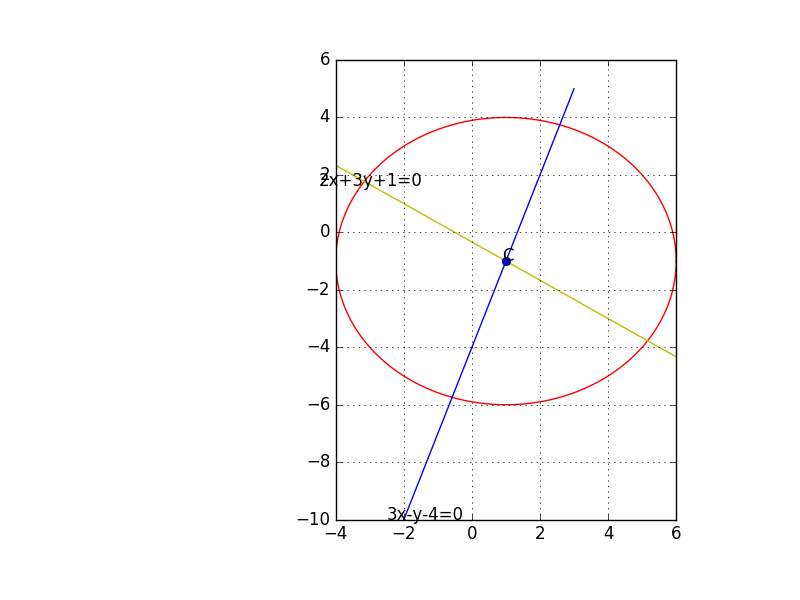
\includegraphics[width=\linewidth]{presentation.png}
\end{figure}


\end{frame}
\end{document}